\documentclass[10pt,twocolumn,letterpaper]{article}

\usepackage{cvpr}
\usepackage{times}
\usepackage{epsfig}
\usepackage{graphicx}
\usepackage{amsmath}
\usepackage{amssymb}
\usepackage[breaklinks=true,bookmarks=false]{hyperref}
\usepackage{color}
\usepackage{indentfirst}
\usepackage{listings}
\definecolor{codegreen}{rgb}{0,0.6,0}
\definecolor{codegray}{rgb}{0.5,0.5,0.5}
\definecolor{codepurple}{rgb}{0.58,0,0.82}
\definecolor{backcolour}{rgb}{0.95,0.95,0.92}


\lstdefinestyle{mystyle}{
  backgroundcolor=\color{backcolour},
  commentstyle=\color{codegreen},
  keywordstyle=\color{magenta},
  numberstyle=\tiny\color{codegray},
  stringstyle=\color{codepurple},
  basicstyle=\footnotesize,
  breakatwhitespace=false,
  breaklines=true,
  captionpos=b,
  keepspaces=true,
  numbers=left,
  numbersep=5pt,
  showspaces=false,
  showstringspaces=false,
  showtabs=false,
  tabsize=2
}
\lstset{style=mystyle}
\cvprfinalcopy % *** Uncomment this line for the final submission

\def\cvprPaperID{****} % *** Enter the CVPR Paper ID here
\def\httilde{\mbox{\tt\raisebox{-.5ex}{\symbol{126}}}}

% Pages are numbered in submission mode, and unnumbered in camera-ready
%\ifcvprfinal\pagestyle{empty}\fi
\setcounter{page}{4321}
\begin{document}

%%%%%%%%% TITLE
\title{
Computer Vision Course Project Report\\ 
Gambody
}

\author{Rong Yuyang, Cai Jianxion, Li Ziyue, Huang Jingyi, Pang Anqi\\
School of Information Science and Technolody\\
ShanghaiTech University\\
{\tt\small \{rongyy, caijx, lizy, huangjy, pangaq\}@shanghaitech.edu.cn}
}

\maketitle

\begin{abstract}

\end{abstract}
\section{Introduction}
\section{Related Work}
\section{Our Approach}
	\subsection{Mask Generation}
		\par We generate mask by taking a photo of a pose and the background first. 
		Then we substract the image to get the binary mask of the pose. 
		We also use Openpose to generate a skeleton data and image.
		\begin{figure}[h]
			\centering
			
\includegraphics[width=0.45\linewidth]{./Pic/Approach_Mask_back}
			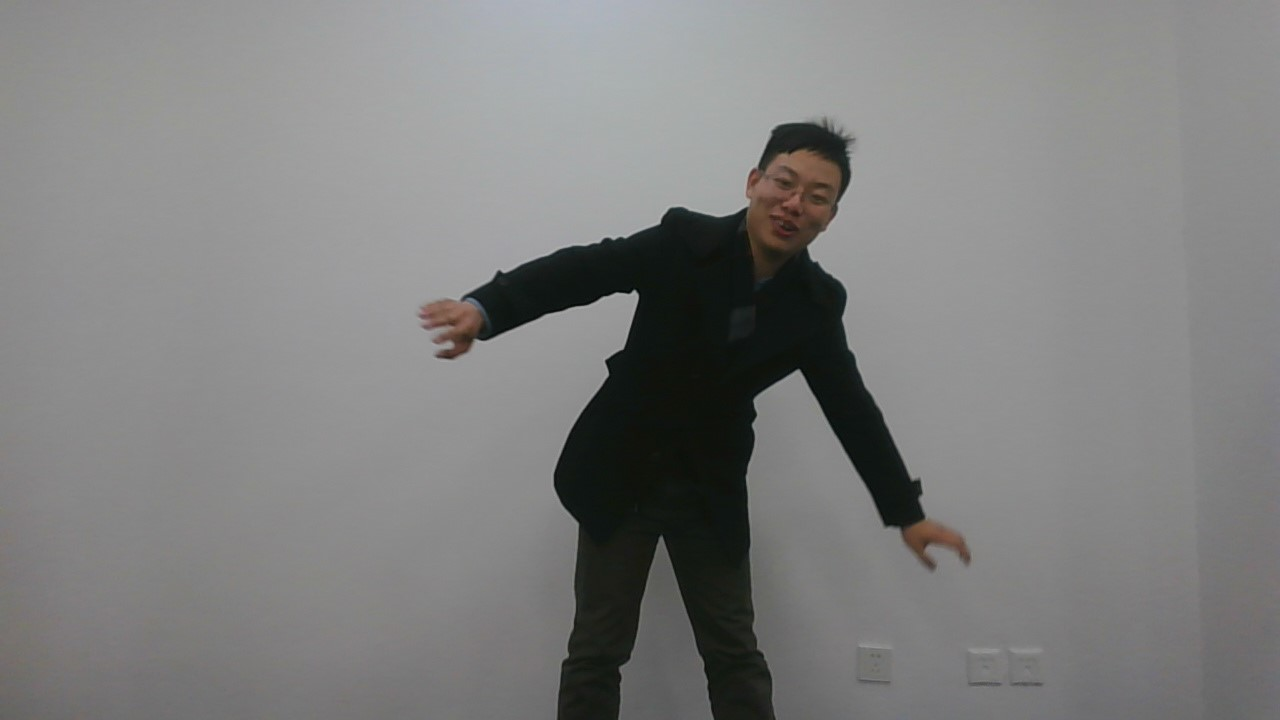
\includegraphics[width=0.45\linewidth]{./Pic/Approach_Mask_pose}
			\caption{Initial images given}
		\end{figure}
		\begin{figure}[h]
			\centering
			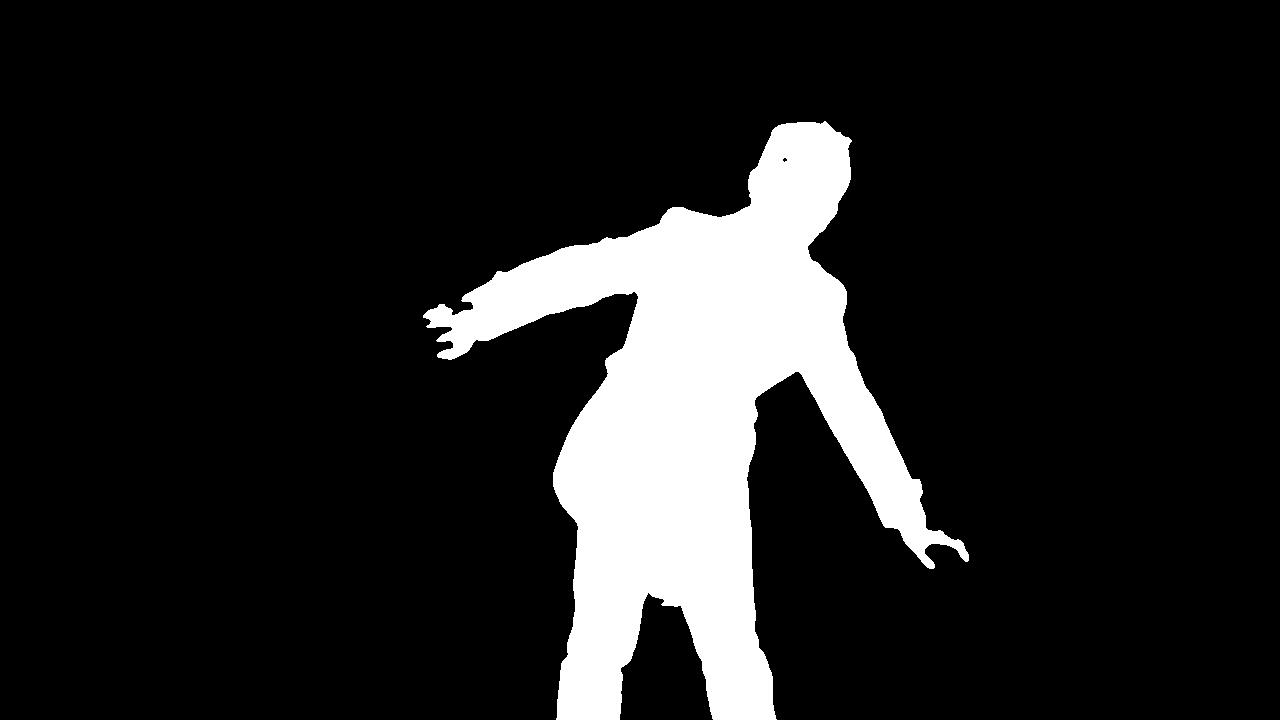
\includegraphics[width=0.9\linewidth]{./Pic/Approach_Mask_binary_mask}
			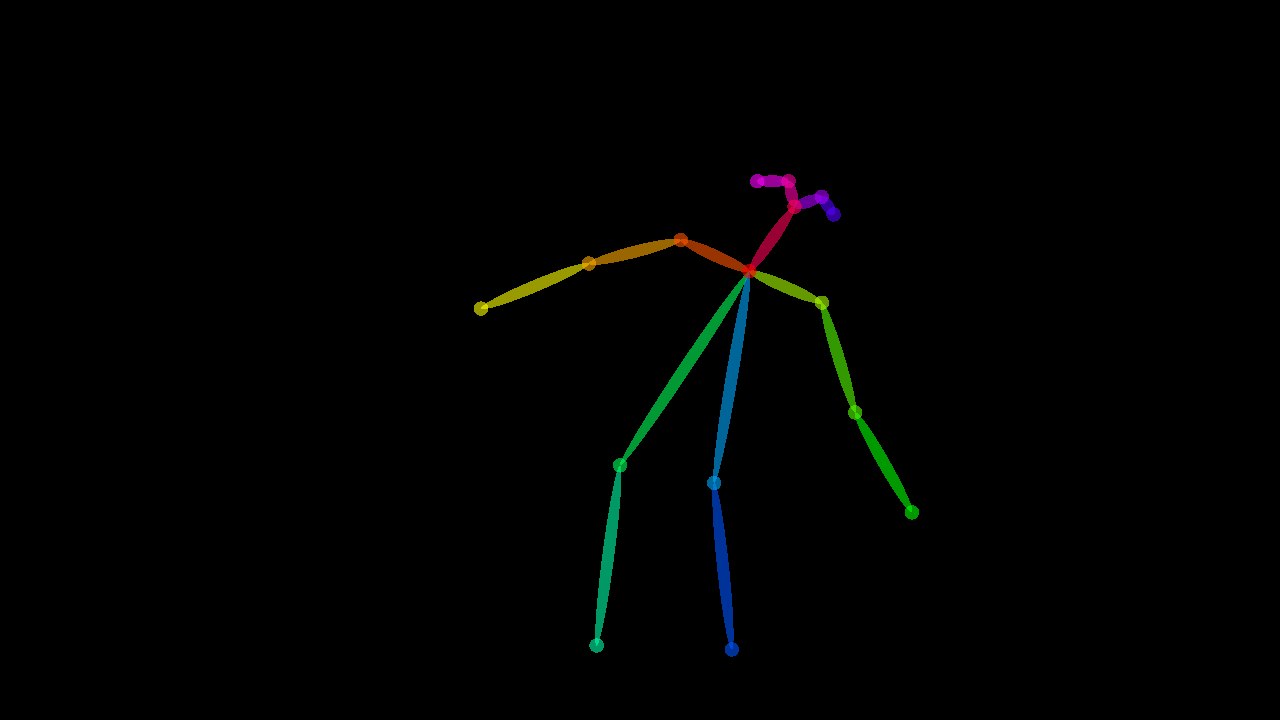
\includegraphics[width=0.9\linewidth]{./Pic/Approach_Mask_skeleton}
			\caption{Mask generated}
		\end{figure}
	\subsection{Version One}
	\subsection{Openpose\cite{cao2017realtime}}

		\subsubsection{Json}
	\subsection{Noise}
\section{Experiment}
	\subsection{Weight on Skeleton}
	\subsection{Noise Cancellation Parameter}
\section{Conclusion}


{\small
\bibliographystyle{ieee}
\bibliography{report}
}
\end{document}
